\section{Introduction}\label{intro:section}
For a finite set $U\subset\R^2$, let
\[
 u(U)=\#\{\{x,y\}\subset U:|x-y|=1\},\qquad
 u(n)=\max_{|U|=n}u(U),
\]
where the pairs are unordered and the distance is Euclidean. The unit
distance problem of Erd\H{o}s \cite{Erdos1946} asks for the order of
growth of $u(n)$. Our main result is the following.

\begin{theorem}\label{thm:main}
There are finite sets $U_j\subset\R^2$, with $|U_j|\to\infty$, such that
\[
 \frac{u(U_j)}{|U_j|^{1.043171}}\longrightarrow\infty.
\]
In particular, $u(n)\ge n^{1.043171}$ for arbitrarily large integers $n$.
\end{theorem}

The theorem concerns an unbounded sequence of cardinalities; it asserts
nothing for every sufficiently large $n$. Its proof uses no unproved
hypothesis, such as the generalized Riemann hypothesis, but it is
computer-assisted: finite facts about the tower, a census of primes, and
many numerical inequalities, among them enclosures of the values of $576$
$L$-functions near $s=1$, are verified by exact computation and interval
arithmetic (Subsection~\ref{intro:code}).

The largest exponent previously claimed in a manuscript, $1.04273$, is in
the author's paper \cite{Naslund04273}. The present paper keeps its
method and most of its construction, and it repeats the parts that are
used, so that it can be read on its own. It differs in three places,
described in Subsection~\ref{intro:new}: one of the local conditions of
the tower, the bound for the relative zeta value, and the weights at the
selected primes (the primes used for equal-norm choices,
Subsection~\ref{intro:outline}).

\subsection{Background}\label{intro:background}
Erd\H{o}s \cite{Erdos1946} showed that a suitable section of a scaled
integer lattice gives
\[
 u(n)\ge n^{1+c_0/\log\log n}
\]
for some $c_0>0$ and arbitrarily large $n$, and he conjectured that this is
essentially optimal \cite{Erdos1946,Erdos1994}. The best upper bound,
\[
 u(n)=O(n^{4/3}),
\]
is due to Spencer, Szemer\'edi and Trotter
\cite{SpencerSzemerediTrotter1984}; Sz\'ekely \cite{Szekely1997} gave a
proof by crossing numbers.

In $2026$ a team at OpenAI \cite{OpenAI2026} disproved Erd\H{o}s's
conjecture. They constructed sets with $u(U)\ge|U|^{1+\delta}$ for a
fixed $\delta>0$ and arbitrarily large $|U|$, replacing the integer
lattice by ideal lattices in number fields of large degree and small
root discriminant $\rd(M)=|\Delta_M|^{1/[M:\Q]}$ ($\Delta_M$ the
discriminant). Alon, Bloom, Gowers, Litt, Sawin, Shankar, Tsimerman,
Wang and Wood \cite{Alon2026} simplified the argument, and Sawin
\cite{Sawin2026} made every step explicit and reached the exponent
$1.014114$. Improvements followed in online discussions
\cite{ErdosProblems90,SpiderduckpigMO2026,NaslundMO2026}, and the
author's manuscript \cite{Naslund0358} recorded $1.0358324$. The paper
\cite{Naslund04273} reached $1.04273$ with a tower over
$\Q(\sqrt{241})$ and quadratic extensions $K/F$ of \emph{mixed
signature}, that is, with $F$ having both real and complex places.
Table~\ref{intro:table-bounds} lists the explicit exponents, and the
repository \cite{TaoConstants84a} records further bounds posted online.

\begin{table}[htbp]
\centering
\caption{Explicit lower bounds $u(n)\ge n^{1+\delta}$ for arbitrarily
large $n$, in increasing order. The exponents are rounded down and
constant factors are omitted. Apart from Erd\H{o}s's, none of these
bounds had appeared in a refereed journal when this paper was written.}
\label{intro:table-bounds}
\small
\begin{tabular}{@{}llll@{}}
\toprule
Exponent & Source & Main new input & Kind of source\\
\midrule
$1+c_0/\log\log n$ & Erd\H{o}s \cite{Erdos1946} & integer lattice & journal\\
$1+\delta$, $\delta>0$ & OpenAI \cite{OpenAI2026} & ideal lattices from class field towers & manuscript\\
$1+6\cdot10^{-38}$ & Alon et al.\ \cite{Alon2026} & simplified argument & preprint\\
$1.014114$ & Sawin \cite{Sawin2026} & explicit and sharpened criterion & preprint\\
$1.015263$ & Emmerich \cite{Emmerich2026} & optimized parameters & preprint\\
$1.031185$ & Emmerich, Cordella \cite{EmmerichCordella2026} & extended range of primes & online certificate\\
$1.031849$ & mlewko \cite{ErdosProblems90} & finite data found by ChatGPT & forum post\\
$1.0333487$ & spiderduckpig \cite{SpiderduckpigMO2026} & weighted Zassenhaus count & online post\\
$1.0358324$ & Naslund \cite{Naslund0358,NaslundMO2026} & covolume counting, dyadic & manuscript,\\
 & & ramification, fixed-subfield Euler products & online post\\
$1.04273$ & Naslund \cite{Naslund04273} & tower over $\Q(\sqrt{241})$, mixed signature & manuscript\\
$1.042901$ & \cite{NaslundCode4317} & Frobenius cap above $41$ instead of at $7$ & research record\\
$1.043171$ & this paper & see Subsection~\ref{intro:new} & \\
\bottomrule
\end{tabular}
\end{table}

\subsection{The construction in outline}\label{intro:outline}
The construction carries Erd\H{o}s's lattice argument to number fields
of large degree. Let $K$ be such a field, of degree $2d$, with an
involution $\iota$ whose fixed field is $F$. We take the points of a
translated ideal lattice of $K$ that lie in a bounded region of
$K\otimes\R$. A complex embedding in which $\iota$ acts as complex
conjugation maps them injectively to the plane. It sends every
difference of relative norm one over $F$ to a unit vector, so two points
whose difference has relative norm one are at distance one. The
exponent is then set by a balance between four quantities, each
normalized as $d^{-1}$ times the logarithm of a count. First,
equal-norm choices: if a prime $\mathfrak p$ of $F$ splits in $K$ as
$\mathfrak P\cdot\iota\mathfrak P$, the $k+1$ ideals
$\mathfrak P^j(\iota\mathfrak P)^{k-j}$, $0\le j\le k$, all have
relative norm $\mathfrak p^k$; the primes used in this way are the
\emph{selected primes} (they lie above the selected primes of $B$ of
Definition~\ref{an:selected-def}). Second, ideal classes: keeping the products of
such ideals that lie in one class of $\Cl(K)$ modulo the image of
$\Cl(F)$ loses at most a factor equal to the order of that quotient
(Lemma~\ref{geo:selection}). Through the class-number formula, this loss
is governed by the root discriminant $\lambda=\rd(K)$ of $K$
(Definition~\ref{tw:rd}), which equals that of $F$ because $K/F$ will be
unramified at the finite places, and by the
\emph{relative zeta value} $L_F(1)$, where $L_F(s)=\zeta_K(s)/\zeta_F(s)$.
Third, the region: its shape decides how many pairs of points with
difference of relative norm one lie in it, and its volume fixes the
number of points. Fourth, density: using a prime $\mathfrak p$ with
exponent $k$ makes the ideal lattice denser by the factor
$\mathrm N\mathfrak p^k$, which costs $\delta k\log\mathrm N\mathfrak p$ before
division by $d$.

Quantitatively, suppose that such fields exist with $d\to\infty$, a
fixed root discriminant $\lambda$, and selected primes of fixed local
types (ramification index and residue degree, Definition~\ref{tw:type}). Let $(b,c)$ be the signature of $F$, so that $d=b+2c$, and put
$\theta=c/d$. If $C$ is an upper bound for $d^{-1}\log L_F(1)$, then
the exponent $1+\delta$ is attained when the \emph{margin}
\begin{equation}\label{intro:margin}
 \frac1d\sum_{\mathfrak p}\log\mathcal F_{\delta,\mathfrak p}
 -\Bigl(\frac12-\delta\Bigr)\log\lambda-C+(1-\delta)\log2
 +(1-\theta)\log\pi+(1-2\theta)J_\R+\theta J_\C
\end{equation}
is bounded below by a positive constant. Here the sum runs over the
selected primes of $F$, and $\mathcal F_{\delta,\mathfrak p}$ is the value
of the local functional of Definition~\ref{fw:local-functional} at the
weight function placed at $\mathfrak p$, a \emph{shell profile}
(Definition~\ref{fw:shell-profile}); for an unweighted profile used with exponent $k$
at a prime of norm $Q$ it is $(k+1)Q^{-\delta k}$. The numbers $J_\R$ and
$J_\C$ are functionals of the profiles at the real and complex places of
$F$ (Definition~\ref{geo:profiles}). This is
Proposition~\ref{fw:transfer}, the geometric transfer with shell
profiles; Section~\ref{sec:certificate} proves that the margin is
positive at $\delta=\deltastar$.

The fields come from a tower: a pro-$2$ extension of
$B=\Q(\sqrt{241})$ with restricted ramification and prescribed local
Galois groups. Its Galois group is the \emph{tower group} $G_B$
(Definition~\ref{tw:GB}), a pro-$2$ group; we write $(D_nG_B)_{n\ge1}$ for its
Zassenhaus filtration and $\operatorname{gr}_nG_B=D_nG_B/D_{n+1}G_B$ for its
graded pieces (recalled at the start of Section~\ref{tw:tower}). The tower is
infinite because its Golod--Shafarevich function
$P_B$ of \eqref{tw:PB} takes a negative value
\cite{GolodShafarevich,HajirMaireRamakrishna2021Cutting}. Its fields
have $\lambda=2^{9/4}\sqrt{3615}\approx286.0$, the field $F$ is the fixed
field of one complex conjugation $\iota_1$, whose conjugacy class in
$G_B/D_4G_B$ has $2^{15}$ elements (Lemma~\ref{tw:retained-quotient}(c)),
which forces $b/d\le2^{-16}$ and $\theta\ge\theta_*=\thetastar$
(Theorem~\ref{tw:field-family}).

\subsection{The structure of the proof}\label{intro:structure}
Figure~\ref{fig:structure} shows how the main statements depend on each
other. The proof has four parts: Parts (II)--(IV) apply to the fields of
Part (I); Parts (II) and (III) are independent of each other and meet in
the final inequality of Part (IV).
\begin{enumerate}
\item[(I)] \emph{The fields} (Section~\ref{tw:tower}). A presentation of the
 Galois group of the maximal pro-$2$ extension of $B$ unramified outside
 $2,3,5$, the local conditions, and the Golod--Shafarevich criterion show
 that the tower is infinite (Proposition~\ref{tw:infinite}); the graded
 pieces of its Zassenhaus filtration (Lemmas~\ref{tw:quadratic-layer}
 and~\ref{tw:retained-quotient}) give the root discriminant, the local
 types and the signature of its fields (Theorem~\ref{tw:field-family}).
\item[(II)] \emph{The relative zeta value} (Sections~\ref{gf:section}--\ref{ce:section}).
 A limit lemma (Lemma~\ref{an:limit}) and the signed kernel inequality
 (Proposition~\ref{an:signed}) reduce $d^{-1}\log L_F(1)$ to values of a zeta
 function at real points $\sigma_j>1$ and to \emph{floors}: lower bounds for
 the residue degrees of the \emph{free} primes of $B$, those other than the
 selected ones (Definitions~\ref{an:selected-def} and~\ref{an:floor-def}). The
 dihedral quotients of $G_B$ supply the floors, through a census of primes
 (Proposition~\ref{dh:census}), and a field $\EW$ of degree $8192$
 (Definition~\ref{dh:W}), whose zeta function factors into the
 $L$-functions of Lemma~\ref{dh:EW}. Their values
 (Proposition~\ref{lv:values}) and the kernel (Lemmas~\ref{ce:kernel}
 and~\ref{ce:values}) give the bound $C_{\rm eff}=\Ceff$ for
 $d^{-1}\log L_F(1)$ (Theorem~\ref{an:ceiling}).
\item[(III)] \emph{The planar sets} (Sections~\ref{geo:section}--\ref{pf:section}).
 A mass formula for ideal lattices (Proposition~\ref{geo:mass}), the class
 selection (Lemma~\ref{geo:selection}) and local and archimedean profiles
 give the transfer Proposition~\ref{fw:transfer}: for fields as in (I), the
 exponent $1+\delta$ is attained when the margin \eqref{intro:margin} is
 positive.
\item[(IV)] \emph{The certificate} (Section~\ref{sec:certificate}). Exact
 checks and interval enclosures of the local functionals, the profile
 integrals and the margin at $\delta=\deltastar$, with $C=C_{\rm eff}$ from
 (II) (Theorem~\ref{an:ceiling}), complete the proof of Theorem~\ref{thm:main}.
\end{enumerate}
The dependency index (Appendix~\ref{dep:section}) lists, for each numbered
statement, the numbered statements that it or its proof cites and the
statements that cite it.

% Generated by tools/depgraph.py -- do not edit by hand.
\begin{figure}[tp]
\centering
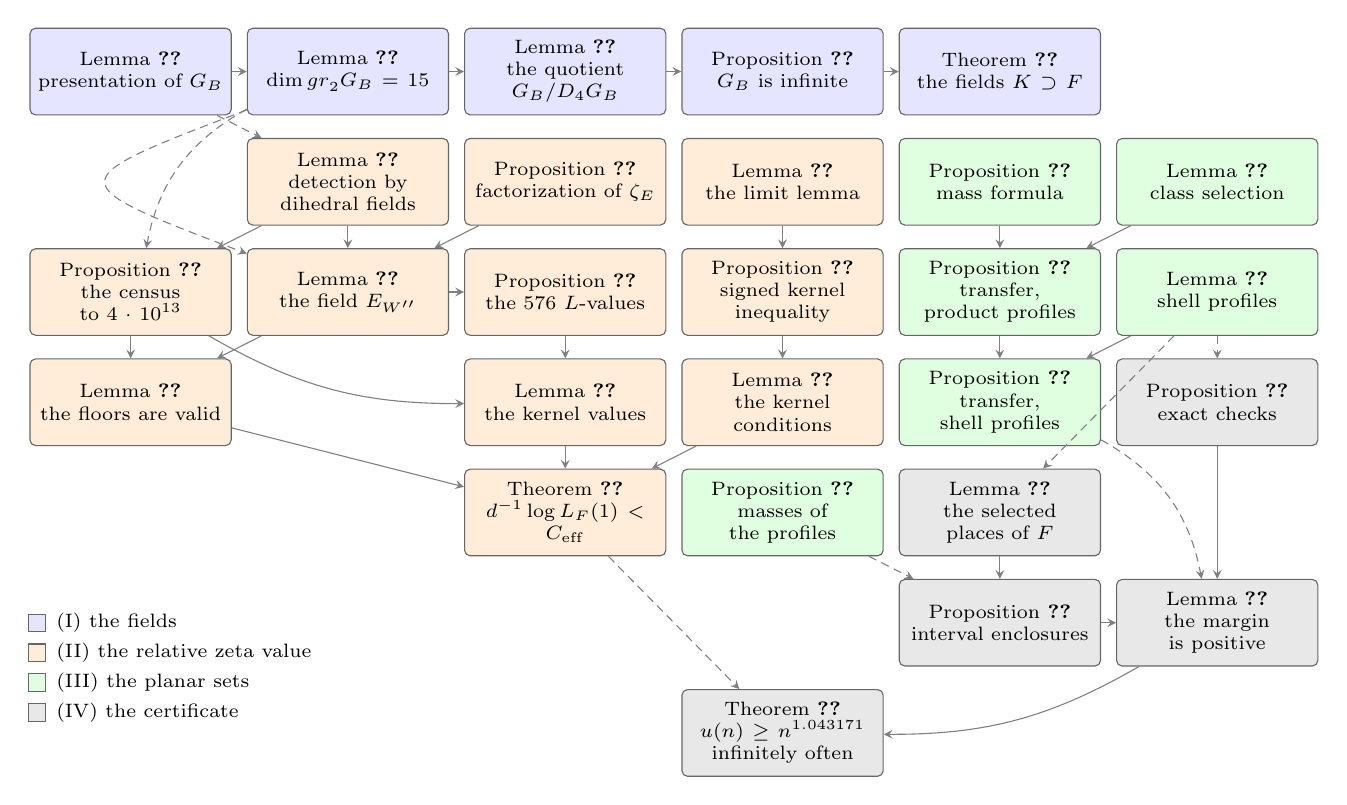
\begin{tikzpicture}[x=1cm,y=1cm,>=stealth,
 box/.style={draw=black!60,rounded corners=2pt,align=center,font=\scriptsize,
  execute at begin node={\hyphenpenalty=10000\exhyphenpenalty=10000},
  inner sep=1.5pt,minimum height=1.10cm,text width=2.45cm}]
\node[box,fill=blue!10] (tw-GB-presentation) at (0.000,0.000) {Lemma~\ref*{tw:GB-presentation}\\ presentation of $G_B$};
\node[box,fill=blue!10] (tw-quadratic-layer) at (2.760,0.000) {Lemma~\ref*{tw:quadratic-layer}\\ $\dim\operatorname{gr}_2G_B=15$};
\node[box,fill=blue!10] (tw-retained-quotient) at (5.520,0.000) {Lemma~\ref*{tw:retained-quotient}\\ the quotient $G_B/D_4G_B$};
\node[box,fill=blue!10] (tw-infinite) at (8.280,0.000) {Proposition~\ref*{tw:infinite}\\ $G_B$ is infinite};
\node[box,fill=blue!10] (tw-field-family) at (11.040,0.000) {Theorem~\ref*{tw:field-family}\\ the fields $K\supset F$};
\node[box,fill=orange!15] (dh-detection) at (2.760,-1.400) {Lemma~\ref*{dh:detection}\\ detection by dihedral fields};
\node[box,fill=orange!15] (gf-factorization) at (5.520,-1.400) {Proposition~\ref*{gf:factorization}\\ factorization of $\zeta_E$};
\node[box,fill=orange!15] (an-limit) at (8.280,-1.400) {Lemma~\ref*{an:limit}\\ the limit lemma};
\node[box,fill=orange!15] (dh-census) at (0.000,-2.800) {Proposition~\ref*{dh:census}\\ the census to $4\cdot10^{13}$};
\node[box,fill=orange!15] (dh-EW) at (2.760,-2.800) {Lemma~\ref*{dh:EW}\\ the field $E_{W''}$};
\node[box,fill=orange!15] (lv-values) at (5.520,-2.800) {Proposition~\ref*{lv:values}\\ the $576$ $L$-values};
\node[box,fill=orange!15] (an-signed) at (8.280,-2.800) {Proposition~\ref*{an:signed}\\ signed kernel inequality};
\node[box,fill=orange!15] (dh-floors-valid) at (0.000,-4.200) {Lemma~\ref*{dh:floors-valid}\\ the floors are valid};
\node[box,fill=orange!15] (ce-values) at (5.520,-4.200) {Lemma~\ref*{ce:values}\\ the kernel values};
\node[box,fill=orange!15] (ce-kernel) at (8.280,-4.200) {Lemma~\ref*{ce:kernel}\\ the kernel conditions};
\node[box,fill=orange!15] (an-ceiling) at (5.520,-5.600) {Theorem~\ref*{an:ceiling}\\ $d^{-1}\log L_F(1)<C_{\rm eff}$};
\node[box,fill=green!12] (geo-mass) at (11.040,-1.400) {Proposition~\ref*{geo:mass}\\ mass formula};
\node[box,fill=green!12] (geo-selection) at (13.800,-1.400) {Lemma~\ref*{geo:selection}\\ class selection};
\node[box,fill=green!12] (geo-transfer) at (11.040,-2.800) {Proposition~\ref*{geo:transfer}\\ transfer, product profiles};
\node[box,fill=green!12] (fw-shell-lemma) at (13.800,-2.800) {Lemma~\ref*{fw:shell-lemma}\\ shell profiles};
\node[box,fill=green!12] (fw-transfer) at (11.040,-4.200) {Proposition~\ref*{fw:transfer}\\ transfer, shell profiles};
\node[box,fill=green!12] (pf-mass) at (8.280,-5.600) {Proposition~\ref*{pf:mass}\\ masses of the profiles};
\node[box,fill=gray!18] (cert-exact) at (13.800,-4.200) {Proposition~\ref*{cert:exact}\\ exact checks};
\node[box,fill=gray!18] (cert-places) at (11.040,-5.600) {Lemma~\ref*{cert:places}\\ the selected places of $F$};
\node[box,fill=gray!18] (cert-enclosures) at (11.040,-7.000) {Proposition~\ref*{cert:enclosures}\\ interval enclosures};
\node[box,fill=gray!18] (cert-lower-margin) at (13.800,-7.000) {Lemma~\ref*{cert:lower-margin}\\ the margin is positive};
\node[box,fill=gray!18] (thm-main) at (8.280,-8.400) {Theorem~\ref*{thm:main}\\ $u(n)\ge n^{1.043171}$ infinitely often};
\draw[->,black!50,densely dashed] (an-ceiling) -- (thm-main);
\draw[->,black!50] (an-limit) -- (an-signed);
\draw[->,black!50] (an-signed) -- (ce-kernel);
\draw[->,black!50] (ce-kernel) -- (an-ceiling);
\draw[->,black!50] (ce-values) -- (an-ceiling);
\draw[->,black!50] (cert-enclosures) -- (cert-lower-margin);
\draw[->,black!50] (cert-exact) -- (cert-lower-margin);
\draw[->,black!50] (cert-lower-margin) to[bend left=15] (thm-main);
\draw[->,black!50] (cert-places) -- (cert-enclosures);
\draw[->,black!50] (dh-EW) -- (dh-floors-valid);
\draw[->,black!50] (dh-EW) -- (lv-values);
\draw[->,black!50] (dh-census) to[bend right=15] (ce-values);
\draw[->,black!50] (dh-census) -- (dh-floors-valid);
\draw[->,black!50] (dh-detection) -- (dh-EW);
\draw[->,black!50] (dh-detection) -- (dh-census);
\draw[->,black!50] (dh-floors-valid) -- (an-ceiling);
\draw[->,black!50,densely dashed] (fw-shell-lemma) -- (cert-exact);
\draw[->,black!50,densely dashed] (fw-shell-lemma) -- (cert-places);
\draw[->,black!50] (fw-shell-lemma) -- (fw-transfer);
\draw[->,black!50,densely dashed] (fw-transfer) to[bend left=25] (cert-lower-margin);
\draw[->,black!50] (geo-mass) -- (geo-transfer);
\draw[->,black!50] (geo-selection) -- (geo-transfer);
\draw[->,black!50] (geo-transfer) -- (fw-transfer);
\draw[->,black!50] (gf-factorization) -- (dh-EW);
\draw[->,black!50] (lv-values) -- (ce-values);
\draw[->,black!50,densely dashed] (pf-mass) -- (cert-enclosures);
\draw[->,black!50,densely dashed] (tw-GB-presentation) -- (dh-detection);
\draw[->,black!50] (tw-GB-presentation) -- (tw-quadratic-layer);
\draw[->,black!50] (tw-infinite) -- (tw-field-family);
\draw[->,black!50,densely dashed] (tw-quadratic-layer) .. controls (-0.920,-1.400) .. (dh-EW);
\draw[->,black!50,densely dashed] (tw-quadratic-layer) to[bend right=25] (dh-census);
\draw[->,black!50] (tw-quadratic-layer) -- (tw-retained-quotient);
\draw[->,black!50] (tw-retained-quotient) -- (tw-infinite);
\node[draw=black!60,fill=blue!10,minimum size=0.22cm,inner sep=0pt] at (-1.190,-7.000) {};
\node[anchor=west,font=\scriptsize,inner sep=0pt] at (-0.950,-7.000) {(I) the fields};
\node[draw=black!60,fill=orange!15,minimum size=0.22cm,inner sep=0pt] at (-1.190,-7.380) {};
\node[anchor=west,font=\scriptsize,inner sep=0pt] at (-0.950,-7.380) {(II) the relative zeta value};
\node[draw=black!60,fill=green!12,minimum size=0.22cm,inner sep=0pt] at (-1.190,-7.760) {};
\node[anchor=west,font=\scriptsize,inner sep=0pt] at (-0.950,-7.760) {(III) the planar sets};
\node[draw=black!60,fill=gray!18,minimum size=0.22cm,inner sep=0pt] at (-1.190,-8.140) {};
\node[anchor=west,font=\scriptsize,inner sep=0pt] at (-0.950,-8.140) {(IV) the certificate};
\end{tikzpicture}
\caption{The structure of the proof (Subsection~\ref{intro:structure}). Each box is a numbered statement, coloured by the part of the proof it belongs to. An arrow goes from a statement to each statement whose proof uses it, directly or through statements not shown, except that arrows implied by a chain of drawn arrows are left out; dashed arrows join different parts. The arrows from Theorem~\ref{tw:field-family}, which supplies the fields to which Parts (II)--(IV) apply, are also left out. Appendix~\ref{dep:section} lists the citations between all numbered statements; the notation is collected in Subsection~\ref{intro:notation}.}
\label{fig:structure}
\end{figure}


\subsection{What is new}\label{intro:new}
\emph{A cap above $41$.} The tower of \cite{Naslund04273} bounds the order
of the Frobenius elements by four (a \emph{cap}) at the two primes above
$29$ and at the prime $7$, which is inert in $B$; a capped prime of $B$
that splits into primes of $F$ that split in $K$ becomes selected. The
prime $41$ splits in $B$. Capping one of the two primes above $41$
instead of $7$ costs the same in the Golod--Shafarevich function, and it
does not change the quotient $G_B/D_4G_B$ of the tower group, because
every fourth power lies in $D_4G_B$. But
the selected primes above $41$ have residue field of order $41^4$ instead
of $7^8$, and their contribution to the margin roughly doubles. This
alone gives the exponent $1.042901$ with the bound $C=\ceiling$ of
\cite{Naslund04273}.

\emph{The relative zeta value.} The bound $C$ of \cite{Naslund04273}
compares $\zeta_K$ prime by prime with the zeta function of the Kummer
field $E$, the maximal elementary abelian subextension of the tower,
with $[E:\Q]=512$. A prime of $B$ that splits completely in $E$ is then
counted as if it split completely in $K$; such primes carry about $0.005$
of $C$. We recover most of this through the second graded piece
$\operatorname{gr}_2G_B=D_2G_B/D_3G_B$ of the Zassenhaus filtration, a
vector space over $\Ftwo$ of dimension $15$ (Lemma~\ref{tw:quadratic-layer}):
\begin{enumerate}
\item[(a)] Exactly $27$ linear forms on it are \emph{of dihedral type}
 (Definition~\ref{dh:dihedral-type}):
 they come from quotients of $G_B$ isomorphic to the dihedral group of
 order $8$, each realized by an explicit field of degree $8$ over $B$
 that lies in every field of the tower (Lemmas~\ref{dh:detection}
 and~\ref{dh:beta-exists}). Fifteen
 of them, with independent forms, detect the residue degree of every
 prime of degree one that splits completely in $E$ up to norm
 $4\cdot10^{13}$, except those whose Frobenius lies in $D_3G_B$
 (Subsection~\ref{dh:census-section}).
\item[(b)] The census cannot reach the infinite tail. Seven of the
 dihedral forms span a space $W''$ of dimension four
 (Subsection~\ref{dh:W-section}), and the corresponding field $\EW$, with
 $[\EW:\Q]=8192$, lies in every field of the tower
 (Subsection~\ref{dh:EW-section}). Its zeta function is
 the product of $\zeta_E$, of the squares of $448$ Hecke $L$-functions
 of quadratic characters of quartic fields, and of the fourth powers of
 $128$ Hecke $L$-functions of quadratic characters of octic fields
 (Lemmas~\ref{dh:EW} and~\ref{dh:Lfunctions}). Comparing with $\EW$ instead of $E$ moves fifteen
 sixteenths of the remaining primes, at all norms, from residue degree
 one to two. No larger space of this kind has $L$-functions of degree
 at most~$8$.
\item[(c)] We evaluate these $L$-functions rigorously at real points
 $\sigma$ near $1$, with approximate functional equations whose cut-off
 functions are certified for the four gamma factors that occur
 (Section~\ref{lv:section}); the octic $L$-functions have conductors up
 to $7.2\cdot10^{20}$ and need Dirichlet coefficients up to
 $1.06\cdot10^{11}$.
\item[(d)] The step from $\sigma>1$ to $s=1$ goes through the
 Tsfasman--Vl\u{a}du\c{t} inequality \cite[Proposition~3.1]{TsfasmanVladut2002}
 (Lemma~\ref{an:limit}(b)). Instead of one abscissa, we use a kernel
 $\mathsf K=\sum_jc_jg_{\sigma_j}$, where $g_\sigma(q)=-\log(1-q^{-\sigma})$,
 over $21$ abscissae $\sigma_j$ with coefficients $c_j$ of both signs;
 it dominates the prime-by-prime contribution at $s=1$ up to a multiple
 of the Tsfasman--Vl\u{a}du\c{t} weight
 $w(q)=2\log q\sum_{m\ge1}(q^m+1)^{-1}$ (Proposition~\ref{an:signed}).
\end{enumerate}
Together these lower the bound for $d^{-1}\log L_F(1)$ from $\ceiling$ to
$C_{\rm eff}=\Ceff$ (Theorem~\ref{an:ceiling}). Since the margin falls by
about $23.8$ per unit of $\delta$ and by $1$ per unit of $C$, this is
worth about $0.00027$ in the exponent.

\emph{General shell weights.} The shell profiles of \cite{Naslund04273}
are weighted sums $\sum_{i,j}w_{ij}\mathbf 1_{\mathcal S_i\times
\varpi^{-k}\mathcal S_j}$ over products of \emph{shells}: in a local field
with ring of integers $\mathcal O$ and uniformizer $\varpi$,
$\mathcal S_0=\mathcal O$ and $\mathcal S_i$ ($i\ge1$) is the set of elements
of valuation $-i$, and $k$ is the exponent used at the prime
(Definition~\ref{fw:shell-profile}); the certificate there
used product weights $w_{ij}=x_ix_j$. The local lemma allows any
nonnegative weights (Lemma~\ref{fw:shell-lemma}), and optimized symmetric
$10\times10$ matrices at the primes above $2$, $3$ and $5$ add
$1.5\cdot10^{-5}$ to the margin.

Table~\ref{intro:table-steps} shows the successive certified exponents.
Section~\ref{lim:section} describes the steps that are not needed for
Theorem~\ref{thm:main}, and what is known about the limits of the
method.

\begin{table}[htbp]
\centering\small
\caption{Successive exponents. $C_{\rm eff}$ is the bound for
$d^{-1}\log L_F(1)$ in force; each step keeps the previous ones, and the
profiles are re-optimized at each exponent. Rows marked $*$ are intermediate
certificates, described in Section~\ref{lim:section}; the proof of
Theorem~\ref{thm:main} uses the census, the signed kernel and the field
$\EW$, but not the adaptive dichotomy or the single-abscissa step. The row
marked $\dagger$ was computed during the search, with product shell weights,
and has no witness of its own; every other row has a witness
(Subsection~\ref{intro:code}) and a replay program in the repository.
$E_W$ and $E_{W'}$ are the fields of the spaces $W\subset W'\subset W''$ of
Section~\ref{lim:section}, and ``ceiling over $M$'' means the bound for
$d^{-1}\log L_F(1)$ obtained with $M$ as comparison field.}
\label{intro:table-steps}
\begin{tabular}{@{}p{8.6cm}lr@{}}
\toprule
step & $C_{\rm eff}$ & exponent\\
\midrule
tower of \cite{Naslund04273} & $0.04871285$ & $1.04273$\\
cap above $41$ instead of $7$ & $0.04871285$ & $1.042901$\\
${}^*$adaptive dichotomy (Propositions~\ref{lim:A}, \ref{lim:B}) & $0.048134265$ & $1.042925$\\
${}^*$dihedral census to $10^{12}$ & $0.0471692613$ & $1.042965$\\
${}^*$ceiling over $E_W$, $[E_W:\Q]=2048$, census to $10^{13}$ & $0.0436495$ & $1.043113$\\
${}^*$refined Tsfasman--Vl\u{a}du\c{t} step, one abscissa & $0.0435763$ & $1.043116$\\
${}^*$signed kernel, census to $8.5\cdot10^{14}$ & $0.0433891$ & $1.043124$\\
${}^*$ceiling over $E_{W'}$, $[E_{W'}:\Q]=4096$ & $0.0427163$ & $1.043152$\\
${}^\dagger$ceiling over $\EW$, $[\EW:\Q]=8192$, census to $4\cdot10^{13}$ & $0.0422764$ & $1.043170$\\
general shell weights at $2$, $3$, $5$ & $0.0422764$ & $1.043171$\\
\bottomrule
\end{tabular}
\end{table}

\subsection{Status}\label{intro:status}
The proof of Theorem~\ref{thm:main} is complete as written, but parts of
it rest on computations. Each computation is done by a supplementary
program, named where it is used, in exact arithmetic or in outward-rounded
interval arithmetic, and a replay program reruns the certificate
(Subsection~\ref{intro:code}). The parts new relative to
\cite{Naslund04273} were checked by ten independent reviews by AI agents
in fresh contexts, each given the statements, the arguments and the
programs but not the author's confidence or earlier verdicts. One review
found a material error in an intermediate certificate: thirteen primes
had been credited twice. It was corrected; the exponent of that step did
not change. The other reviews found no error affecting the bounds; their
minor points, among them gaps in the error accounting of the numerical
programs, were fixed. No reviewer recomputed the octic $L$-values
independently, since general-purpose software cannot reach their
conductors; they rest on the method of Section~\ref{lv:section} and its
checks. The cap above $41$ (Section~\ref{tw:tower}) has had two
fresh-context reviews of its argument, but its finite computations have
not had a full independent review. These are automated reviews, not human
peer review.

A Lean formalization \cite{NaslundLean2026} proves the planar conclusion
of \cite{Naslund04273}, with the exponent $1.0427$, from one explicit
inequality for $\zeta_E$; it does not cover the present construction or
its bound for the relative zeta value (Remark~\ref{an:lean-hypothesis}).

\subsection{Organization}\label{intro:organization}
Section~\ref{tw:tower} constructs the tower and proves
Theorem~\ref{tw:field-family}, which supplies the fields.
Section~\ref{gf:section} recalls the Kummer field $E$ and its quadratic
$L$-functions. Section~\ref{an:section} reduces the relative zeta value
to the primes of the fields of the tower, and proves the signed kernel
inequality (Proposition~\ref{an:signed}). Section~\ref{dh:section} treats
the dihedral quotients, the census and the field $\EW$;
Section~\ref{lv:section} evaluates the $L$-functions of $\EW$; and
Section~\ref{ce:section} proves the bound $C_{\rm eff}$
(Theorem~\ref{an:ceiling}). Sections~\ref{geo:section}--\ref{pf:section}
carry out the geometric construction, as in \cite{Naslund04273}, with
general shell weights. Section~\ref{sec:certificate} proves the final
inequality at $\delta=\deltastar$ and completes the proof of
Theorem~\ref{thm:main}. Section~\ref{lim:section} records refinements that
are not used, and the limits of the method. Appendix~\ref{fw-data:section}
lists the optimized shell weights, and the dependency index
(Appendix~\ref{dep:section}) lists, for every numbered statement, the
statements it cites and those that cite it.

\subsection{Notation}\label{intro:notation}
The following symbols keep one meaning throughout the paper. Other letters
($H$, $N$, $\tau$, $\beta$, $\gamma$, $\sigma$, $\nu$, $q$, $s$, $t$, \dots)
are reused in different sections with local meanings, which are defined
where they are introduced.

\smallskip
{\small
\begin{longtable}{@{}>{\raggedright\arraybackslash}p{0.2\textwidth}>{\raggedright\arraybackslash}p{0.53\textwidth}>{\raggedright\arraybackslash}p{0.21\textwidth}@{}}
\toprule
symbol & meaning & defined in\\
\midrule\endhead
$B$, $S$ & $B=\Q(\sqrt{241})$; $S$ the primes of $B$ above $2,3,5$ & Section~\ref{tw:tower}\\
$\mathrm N$ & the absolute norm of an ideal & Section~\ref{tw:tower}\\
$\mathfrak t_1,\dots,\mathfrak t_4$ & the primes of $B$ above $29$ and $41$; the capped primes are $\mathfrak t_1,\mathfrak t_2,\mathfrak t_3$ & Lemma~\ref{tw:base}, Definition~\ref{tw:local-generators}\\
$v_1,v_2$, $\Sigma$ & the real places of $B$; $\Sigma=S\cup\{v_1,v_2\}$ & Section~\ref{tw:tower}\\
$B_S$, $G_S$ & the maximal pro-$2$ extension of $B$ unramified at the finite primes outside $S$, and its Galois group & Section~\ref{tw:tower}\\
$E$ & the Kummer field: the maximal elementary abelian $2$-extension of $B$ in $B_S$, $[E:\Q]=512$ & Section~\ref{tw:tower}\\
$\chi_e$, $\kappa_a$ & the characters of $\Gal(E/B)$, with values $\pm1$ and in $\Ftwo$ & Definitions~\ref{gf:characters}, \ref{tw:elementary-image}\\
$D_nG$, $\operatorname{gr}_nG$ & the Zassenhaus filtration of a pro-$2$ group $G$ and its graded pieces $D_nG/D_{n+1}G$ & Section~\ref{tw:tower}\\
$G_B$, $B_G$, $\overline G_B$ & the tower group; the field $B_G\subset B_S$ of the tower, with $\Gal(B_G/B)=G_B$; and $\overline G_B=G_B/D_4G_B$ & Definition~\ref{tw:GB}\\
$\iota_1$ & a complex conjugation at a place above $v_1$ & Definition~\ref{tw:local-generators}\\
$\rd(M)$, $\lambda$, $\ell$ & root discriminant; $\lambda=2^{9/4}\sqrt{3615}$, the root discriminant of the fields of the tower; $\ell=\log\lambda$ & Definition~\ref{tw:rd}, Theorem~\ref{tw:field-family}\\
$\mathcal K$, $K$, $F$, $d$ & the fields of the tower used; $K\in\mathcal K$, $F=K^{\langle\iota_1\rangle}$, $d=[F:\Q]$ & Definition~\ref{an:family}\\
$(b,c)$, $\theta$, $\theta_*$ & the signature of $F$ ($d=b+2c$), $\theta=c/d$, and the lower bound $\theta_*=\thetastar$ & Theorem~\ref{tw:field-family}\\
$L_F(s)$ & the relative zeta function $\zeta_K(s)/\zeta_F(s)$ & Subsection~\ref{intro:outline}\\
$C$, $C_{\rm eff}$ & an upper bound for $d^{-1}\log L_F(1)$; the bound $C_{\rm eff}=\Ceff$ proved here & Theorem~\ref{an:ceiling}\\
$e_K(\mathfrak p)$, $f_K(\mathfrak p)$ & ramification index and residue degree of a prime $\mathfrak p$ of $B$ in $K/B$ & Section~\ref{an:section}\\
$g_s(q)$, $w(q)$, $\kappa_\infty$ & $g_s(q)=-\log(1-q^{-s})$; $w(q)$ the Tsfasman--Vl\u{a}du\c{t} weight, and $2\kappa_\infty$ the right side of the Tsfasman--Vl\u{a}du\c{t} inequality & Subsection~\ref{an:budget-section}\\
$\beta_q$, $Z(s)$ & limiting densities of primes of norm $q$, and $Z(s)=\sum_q\beta_qg_s(q)$ & Lemma~\ref{an:limit}\\
$Z_{\rm sel}$, $T_{\rm sel}$ & the parts of $Z$ and of the Tsfasman--Vl\u{a}du\c{t} sum from the selected primes & Subsection~\ref{an:selected}\\
selected, free & the selected primes of $B$ (above $2,3,5$ and the capped primes); the other primes of $B$ & Definition~\ref{an:selected-def}\\
$f^0_{\mathfrak p}$, $Y_{\rm fl}$ & floors: lower bounds for the residue degrees of the free primes, conditions (Fl1), (Fl2); the floor sum & Definition~\ref{an:floor-def}\\
$\mathsf K$, $\sigma_j$, $c_j$, $b_{\rm TV}$ & the signed kernel $\sum_jc_jg_{\sigma_j}$ with its $21$ abscissae and coefficients, and its multiplier of $w$ & Proposition~\ref{an:signed}, Definition~\ref{ce:kernel-def}\\
$\mathrm{Dih}_4$, $\psi_o$ & the dihedral group of order $8$; the $27$ forms of dihedral type on $\operatorname{gr}_2G_B$ & Definition~\ref{dh:dihedral-type}, Lemma~\ref{dh:27}\\
$\psi^{\rm c}_1,\dots,\psi^{\rm c}_{15}$ & the census basis of dihedral forms & Definition~\ref{dh:census-basis}\\
$W''$, $\EW$ & the span of seven dihedral forms, $\dim W''=4$, and its field, $[\EW:\Q]=8192$ & Definition~\ref{dh:W}\\
$\delta$, $p$ & the exponent is $1+\delta$; $p=2/(1+\delta)$ is a Lebesgue exponent & Definition~\ref{geo:profiles}\\
$\mathcal S_i$, $\mathcal F_{\delta,\mathfrak p}$ & the shells of a local field; the local functional of the shell profile at $\mathfrak p$ & Definitions~\ref{fw:local-functional}, \ref{fw:shell-profile}\\
$J_\R$, $J_\C$ & the archimedean functionals of the profiles & Definition~\ref{geo:profiles}\\
$(e_r,f_r)$ & for $r=2,3,5,29$ the type of the selected places above $r$; for $r=41$ the
 \emph{effective type} $(2,4)$, a counting device & Definition~\ref{cert:effective-types}\\
\bottomrule
\end{longtable}}

\subsection{Computations and data}\label{intro:code}
The proof uses finite computations: linear algebra over $\Ftwo$ for the
tower and its quotients, exact rational arithmetic for the
Golod--Shafarevich function, a census of primes in C, rigorous
evaluations of $L$-functions in the ball arithmetic of Arb, now part of
FLINT \cite{Johansson2017,FLINT}, and interval arithmetic with directed
rounding for the margin \cite{Mpmath}. PARI/GP \cite{PARI} is used for
the arithmetic of number fields and for independent checks. Each finite
fact is verified by a supplementary program, named in the text where the
fact is used.

The programs and their data are in the directory
\path{papers/0.043171/certificates} of the repository
\cite{NaslundCode4317}. They import, without modifying them, the programs
of \cite{Naslund04273} (directory \path{papers/0.04273/certificates}, in
the version with the interval corrections of October~2, 2026) and of the
41-cap variation (directory \path{papers/0.042901/certificates}), and some
routines of the supplementary archive of the author's earlier note
\cite{Naslund0418235}, whose members are checked against their SHA-256
hashes when the archive is unpacked. A \emph{witness} is a JSON file that
records the exact data of one certificate (the exponent, the bound $C$,
the kernel abscissae and coefficients, the profile parameters and the
shell weights) together with the SHA-256 hashes of the data files it
reads; its replay program recomputes every certified inequality from it.
The witness of Theorem~\ref{thm:main} is
\path{certificates/dihedral/witness_0.043171.json}; it pins the
SHA-256 hashes of $617$ data files, among them all $353$ files that the
certification reads.
The replay program \path{certificates/dihedral/reproduce_w3.py}
regenerates the exports of the number fields with PARI/GP, recomputes
the $L$-values at three of the abscissae and checks the others by hash,
repeats the census on sample ranges and checks the census bins against
an independent classification, reruns the kernel checks and the bound
for the relative zeta value, and recomputes the margin. It takes about
two hours on a machine with sixteen cores. The computations were run
with PARI/GP~2.17.2, python-flint~0.9.0 (FLINT~3.6.0), mpmath~1.3.0,
numpy~2.5.3 and scipy~1.18.1; the census programs need an x86-64
processor with the AVX-512 IFMA instructions.
